\begin{frame}{Aims and motivation} %{{{1

  \begin{columns}
    \begin{column}{0.5\textwidth}
      \begin{itemize}

        \item
          Exploration of defect centres using state-of-the-art ab-initio
          theories.

        \item
          Systematic characterization of defect fingerprints.

        \item
          Search for new defects with tailored properties useful for practical
          applications.

        \item
          Benchmark ab-initio theories with well-known
          experimental data.


      \end{itemize}
    \end{column}
    \begin{column}{0.5\textwidth}
      \begin{center}
        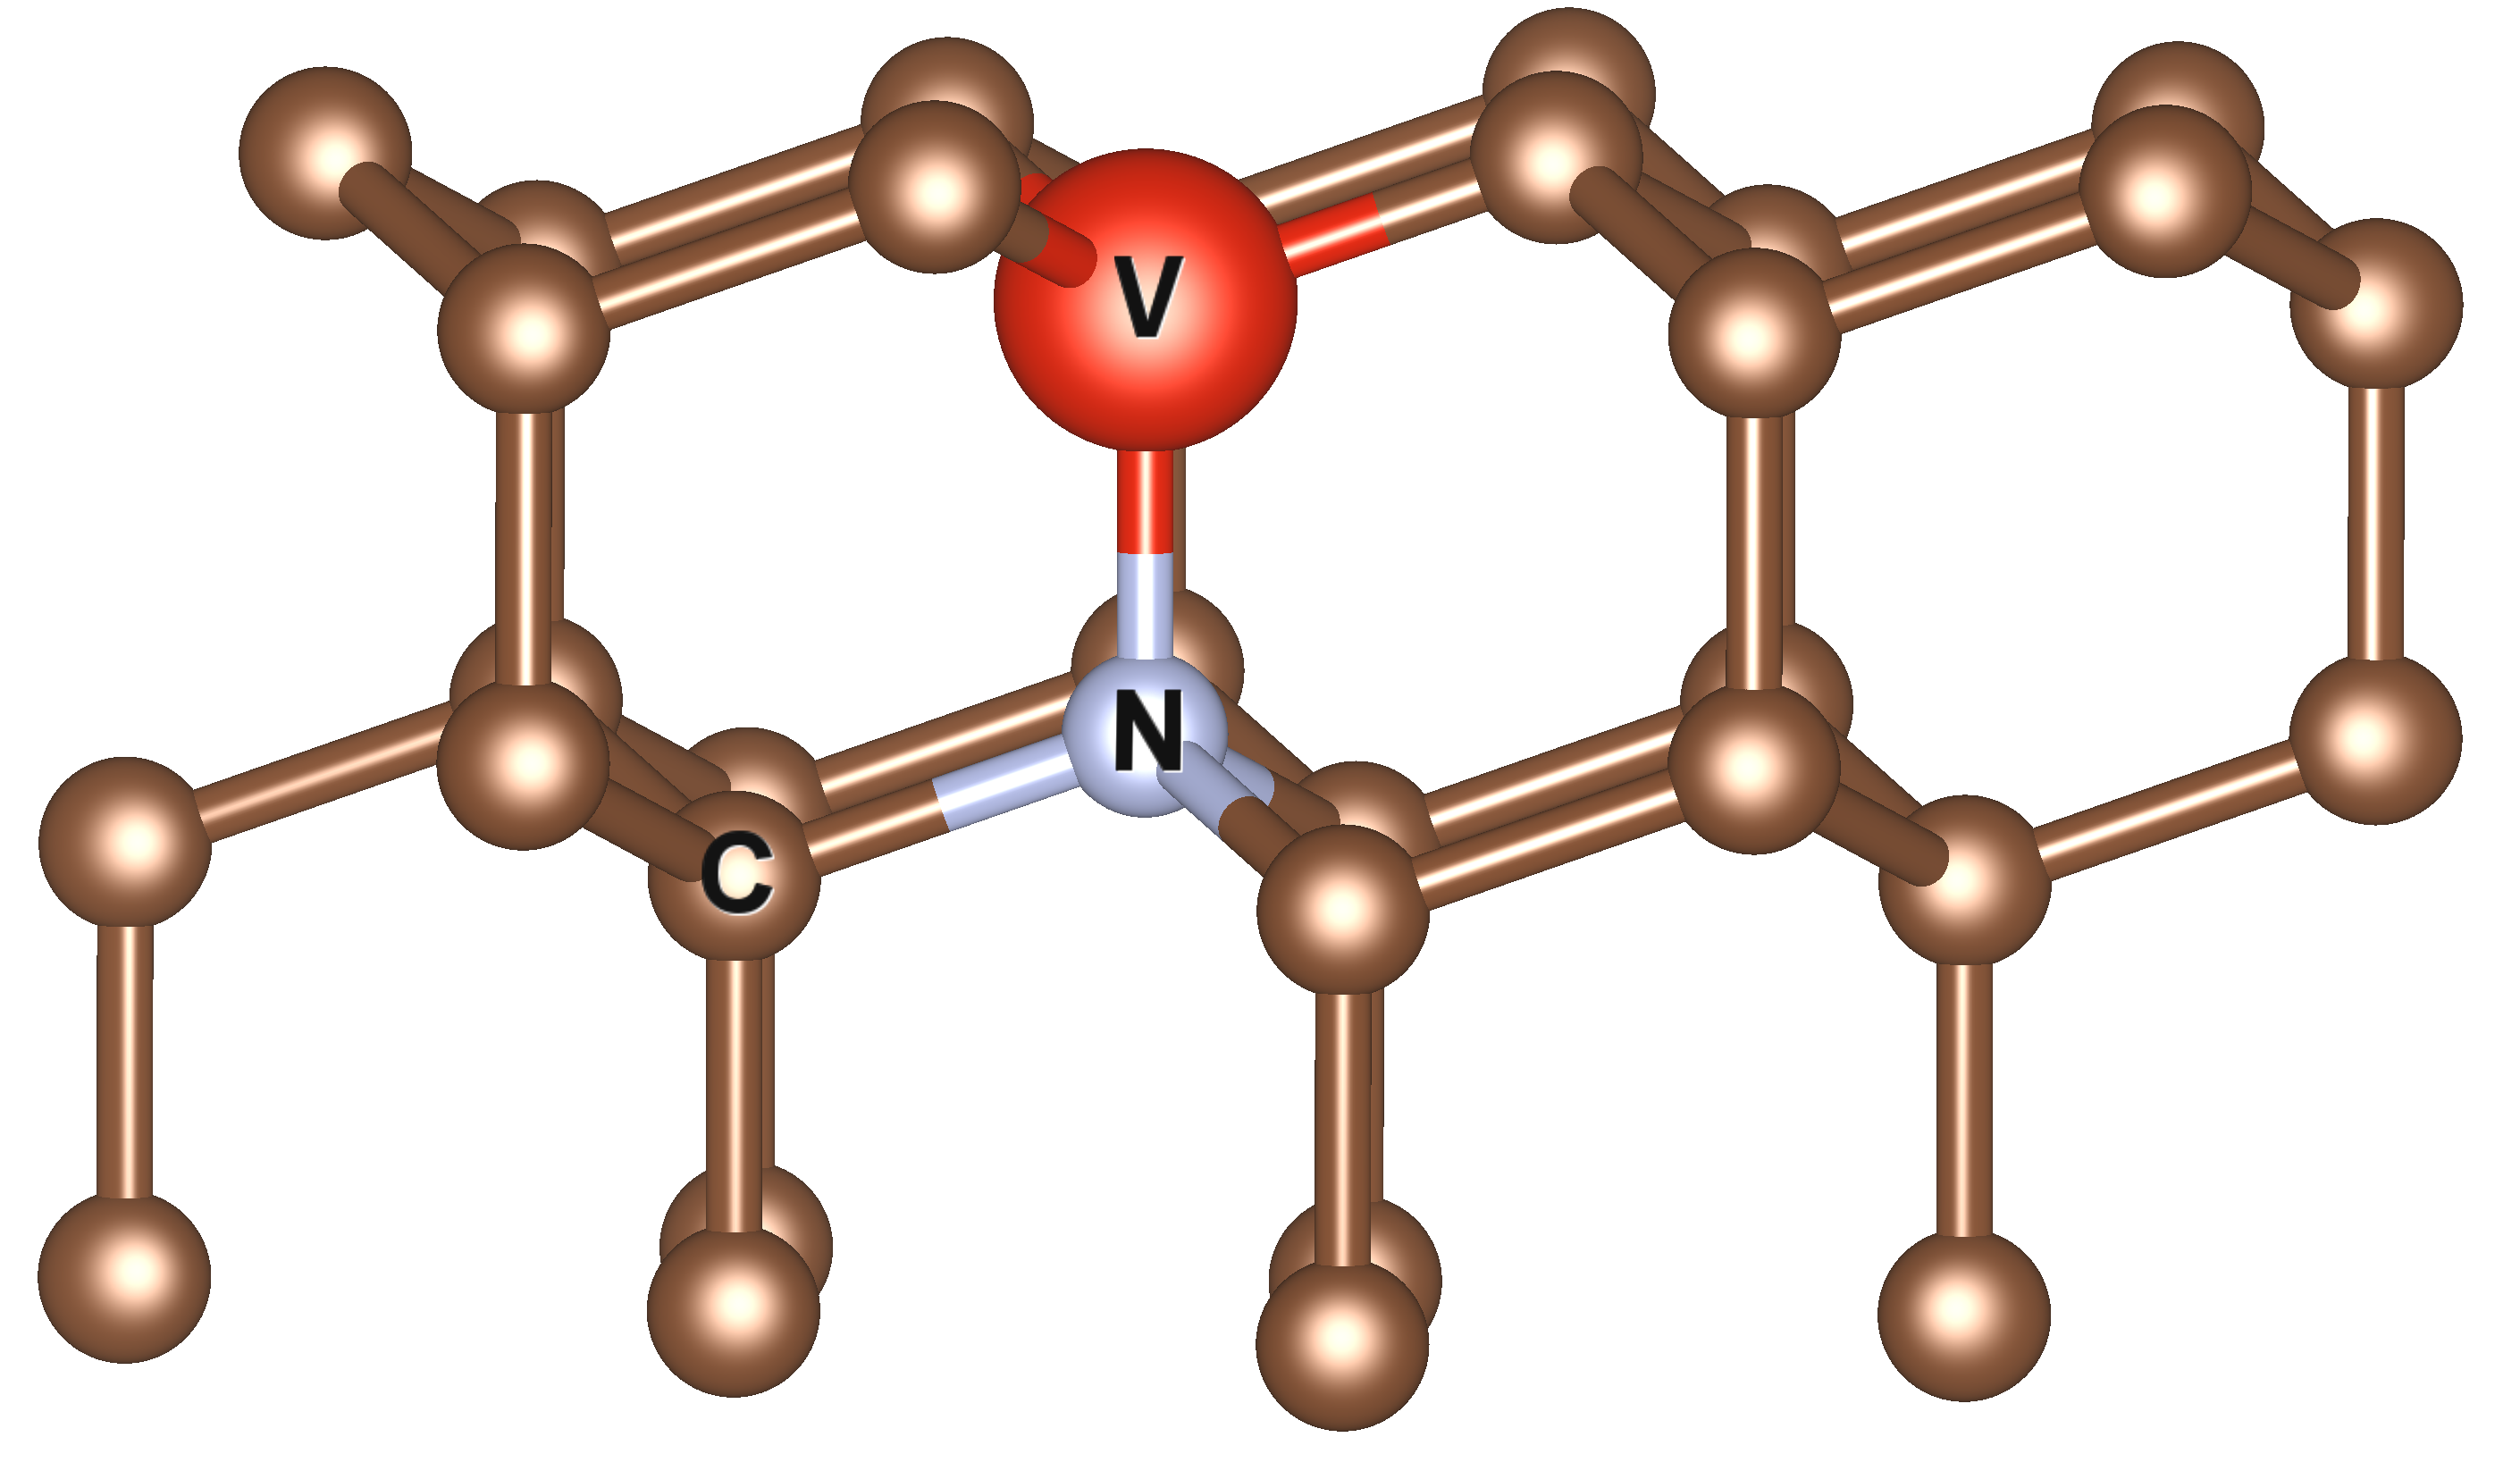
\includegraphics[width=1\textwidth]{images/POSCAR_16_view.png}
      \end{center}
    \end{column}
  \end{columns}

  \note{%

    So the main aim of this work is to computationally
    treat electronic properties of defect centers in diamond
    using state-of-the-art ab initio theories.

    Through this exploration we hope to recover many well-known
    experimentally verified quantities.

    In order to do this we use several purely theoretical
    results to orient our calculations into the right direction.
    (e.g. Markus' Gruppentheorierechnungen)

  }

\end{frame}
